%==============================================================================
%== template for LATEX poster =================================================
%==============================================================================
%
%--A0 beamer slide-------------------------------------------------------------
\documentclass[final]{beamer}

\usepackage{graphicx}
\usepackage{xcolor}
\usepackage[orientation=portrait,size=a0,
            scale=2.2         % font scale factor
           ]{beamerposter}
           
\geometry{
  hmargin=2.5cm, % little modification of margins
}

%
\usepackage[utf8]{inputenc}
\usepackage{ragged2e}

\linespread{1.15}
%
%==The poster style============================================================
\usetheme{sharelatex}

%==Title, date and authors of the poster=======================================
%\title
%[http://python.fossee.in, info@fossee.in, python@fossee%.in] % Conference
%{ % Poster title
%}


%\author{ % Authors
%Author One\inst{1}, Author Two\inst{2}, Author Three\inst{2,3}
%}
%\institute
%[Very Large University] % General University
%{
%\inst{1} Very Large University, Neverland
%\inst{2} Other University, Neverland
%\inst{3} Yet Another University, Neverland
%}
%\date{\today}



\begin{document}
\begin{frame}[t]
%==============================================================================
\begin{multicols}{2}
%==============================================================================
%==The poster content==========================================================
%==============================================================================

\section{What is Python?}

Python is a general purpose, high level, remarkably powerful dynamic
programming language used in a wide variety of application domains.

%% \vskip5ex

\section{Why Python?}
\begin{itemize}
\item {Easy to read and learn}
\item {Free and Open Source}
\item {Useful for scientific computing}
\item {Powerful interactive interpreter}
\item {Extensive scientific libraries}
\item {Well documented}
\end{itemize}

%\vskip5ex

\section{Where can you use Python ?}
\begin{itemize}
\item {Numeric and Symbolic computation}
\item {2D/3D Plotting}
\item {User interfaces}
\item {Parallel computing}
\item {Machine Learning and Image Processing}
\item {Game development}
\item {Web development}
\item {Much more...}  
\end{itemize}

%\vskip5ex


\section{Who uses Python?}
\begin{itemize}
\item {Google}
\item {Yahoo}
\item {Walt Disney}
\item {NASA}
\item {IBM}
\item {YouTube}
\item {nVIDIA}  
\item {Software - Blender, Motion Builder, \\
  Cinema 4D, etc.}
\item {Games - Battlefield 2 by EA sports, \\
  Crystalspace 3D, etc.}
\end{itemize}

\vskip3ex

Python is one of the most popular programming languages today, and
therefore has been included in the CBSE curriculum. It easily performs
tasks that proprietary tools like Matlab and Mathematica offer. Today
leading companies are using Python extensively, hence there are better
job opportunities. Learn Python, and grab the Opportunity!


%% BACK

%% \subsection{How can you learn Python ?}
%% \begin{itemize}
%% \item \justifying {{\bf{Spoken Tutorial}} - A library of spoken tutorials on
%%   'Python' to watch, learn and practice for taking those initial steps
%%   and move on. This is the place that helps you getting started in the
%%   world of FOSS. Learn at your will, any time, anywhere! Learn Python
%%   here - http://python.fossee.in/spoken-tutorials/} \par


%% %\vskip1ex

%% \begin{figure}
%% \centering
%% \fboxsep=0mm%padding thickness
%% \fboxrule=1pt%border thickness
%% \fcolorbox{gray}{white}{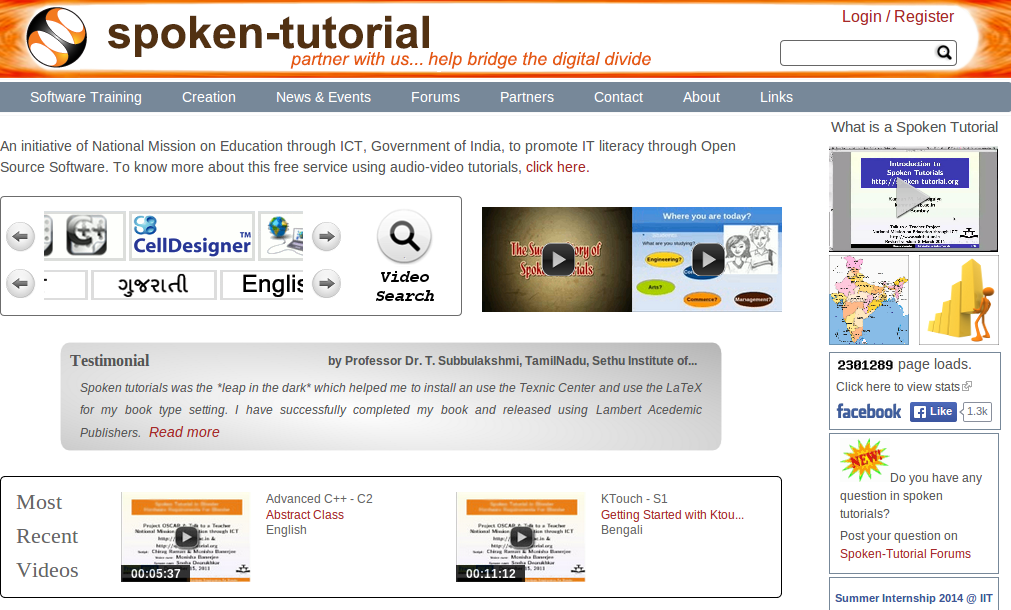
\includegraphics[width=0.99\columnwidth]{spoken-tutorial.png}}
%% \caption{Spoken tutorial website}
%% \end{figure}


%% %\vskip5ex

%% \item \justifying{{\bf{Textbook Companion Activity}} - Learn Python in a
%%   practical and efficient way by contributing to the Python Textbook
%%   Companion activity.  The Textbook Companion activity aims to create
%%   Companions by coding solved examples from Standard textbooks using
%%   Python. Contribute to this activity and earn an honorarium too!  For
%%   more details, please visit -
%%   http://python.fossee.in/textbook-companion-project/}\par

%% %\vskip1ex

%% \begin{figure}
%% \centering
%% \fboxsep=0mm%padding thickness
%% \fboxrule=1pt%border thickness
%% \fcolorbox{gray}{white}{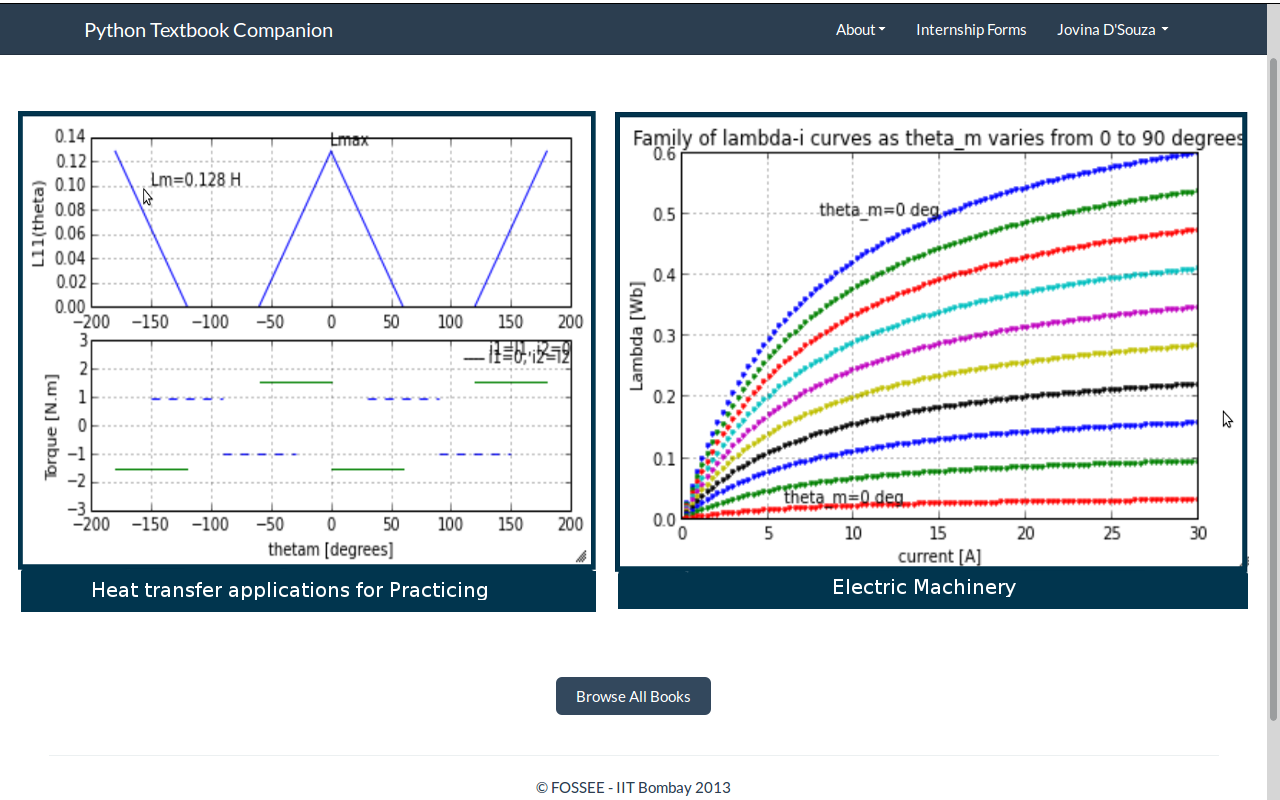
\includegraphics[width=0.99\columnwidth]{tbc.png}}
%% \caption{Python textbook companion}
%% \end{figure}
%% \end{itemize}

%% \vskip5ex

%% \item {{\bf{SELF Workshops}} - Workshops on Python are conducted
%%   remotely by IIT Bombay. These workshops are completely free of cost
%%   and contain high quality material taught by experts in
%%   domain. During these workshops, the participant would use Spoken
%%   tutorials to work on various exercises and examples. Learn Python
%%   and obtain a certificate from IIT Bombay upon successful completion
%%   of a post-workshop test.  Please visit,
%%   http://python.fossee.in/spoken-tutorials/}


%% \subsection{Other python packages}
%% \vskip1ex
%% \begin{figure}
%% \centering
%% 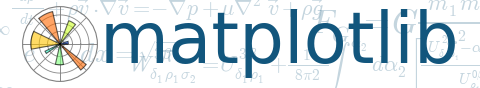
\includegraphics[width=0.7\columnwidth]{matplotlib.png}
%% \caption{Matplotlib}
%% \end{figure}

%% \vskip3ex

%% \begin{figure}
%% \centering
%% 
\includegraphics[width=0.5\columnwidth]{django-logo-positive.png}
%% \caption{Django}
%% \end{figure}

%% \vskip3ex

%% \begin{figure}
%% \centering
%% 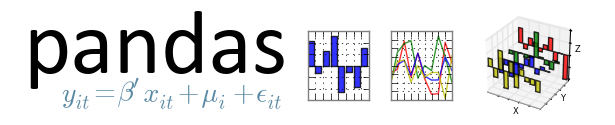
\includegraphics[width=0.7\columnwidth]{pandas_logo.png}
%% \caption{Pandas}
%% \end{figure}

%% \vskip3ex

%% \begin{figure}
%% \centering
%% 
\includegraphics[width=0.5\columnwidth]{scipy.png}
%% \caption{Scipy}
%% \end{figure}

%% \vskip3ex

%% \begin{figure}
%% \centering
%% 
\includegraphics[width=0.4\columnwidth]{sympy.png}
%% \caption{SymPy}
%% \end{figure}

%% \vskip3ex

%% \begin{figure}
%% \centering
%% 
\includegraphics[width=0.6\columnwidth]{IPy_header.png}
%% \caption{IPython}
%% \end{figure}



%% \vskip3ex

%% \begin{figure}
%% \centering
%% 
\includegraphics[width=0.4\columnwidth]{mayavi.png}
%% \caption{Mayavi}
%% \end{figure}

%% \vskip2ex

%% \section{Get in touch}
%% \subsection{About the project}
%% \begin{thebibliography}{99}
%% \bibitem{web} \url{http://fossee.in}
%% \bibitem{web} \url{http://python.fossee.in}
%% \bibitem{web} \url{http://tbc-python.fossee.in}
%% \bibitem{web} \url{http://spoken-tutorial.org}
%% \bibitem{} Email: info@fossee.in, python@fossee.in
%% \end{thebibliography}

%% BACK 

%\subsection{General help and Queries:}
%\begin{thebibliography}{99}
%\bibitem{email} Email: info@fossee.in
%\bibitem{email} Email: python@fossee.in
%\end{thebibliography}
%==============================================================================
%==End of content==============================================================
%==============================================================================
%--References------------------------------------------------------------------
%--End of references-----------------------------------------------------------

\end{multicols}

%==============================================================================
\end{frame}
\end{document}
